% F2 -- (a) page/segment processing; (b) RIS command lifecycle (DESIGN 13.4; WP12).
% Drawn at \textwidth (516 pt). Checked against sremu commit 2a016a6:
%   (a) sremu.engine.scheduler.advance_group (page portion, barrier limit, skip of inactive
%       pages D-6, TX commitment k1 + lookahead, partial page or wait), JobBuilder.render_range
%       (segments at snapshot-interval bounds and per-RX, per-tile switch samples), the RX
%       chain of sremu.engine.streams, Emulator.step (barriers, command statuses), stall
%       report of Emulator.run
%   (b) sremu.engine.barriers (limit to_ticks(t_b + L_min), observation before to_ticks(t_b),
%       actions at t_b + latency >= t_b + L_min, lateness 0 by construction) and
%       sremu.engine.commands (k_{r,j} = to_ticks(t_sw + tau_r), late command:
%       apply_on_arrival moves the switch to t' = max_r(frontier_r/f_r - tau_r); the record
%       keeps k_req, k_applied, lateness and status late_applied)
\documentclass[10pt,tikz,border=0pt]{standalone}
% sremu-figstyle.tex -- shared style of the TikZ diagrams F1 and F2 (WP12; DESIGN 13.4).
% Fonts: Times (newtx), as in the IEEEtran body text; every label is at least 8 pt at print
% size because the diagrams are drawn at their printed width (F1: \columnwidth = 252 pt;
% F2: \textwidth = 516 pt) and included without scaling.
% Colours: Okabe-Ito (colour-blind safe). Every colour coding is doubled by a line style
% (data plane solid, control plane dashed, recording dotted), so the diagrams also read in
% grey scale.
\usepackage[T1]{fontenc}
\usepackage{newtxtext,newtxmath}
\usepackage{tikz}
\usetikzlibrary{arrows.meta,positioning,calc,fit,backgrounds,patterns,decorations.pathreplacing}

\definecolor{okBlack}{HTML}{000000}
\definecolor{okOrange}{HTML}{E69F00}
\definecolor{okSky}{HTML}{56B4E9}
\definecolor{okGreen}{HTML}{009E73}
\definecolor{okYellow}{HTML}{F0E442}
\definecolor{okBlue}{HTML}{0072B2}
\definecolor{okVermillion}{HTML}{D55E00}
\definecolor{okPurple}{HTML}{CC79A7}

\newcommand{\figfont}{\fontsize{8}{9.4}\selectfont\hyphenpenalty=10000\exhyphenpenalty=10000}
\newcommand{\figtitle}{\fontsize{8}{9.4}\selectfont\bfseries}

\tikzset{
  every picture/.style={font=\figfont, line width=0.6pt,
    >={Stealth[length=4.5pt,width=3.6pt,line width=0pt]}},
  box/.style={draw=okBlack, rounded corners=1.5pt, align=center, inner sep=2.5pt,
    fill=white},
  app/.style={box, fill=okSky!18},
  eng/.style={box, fill=okOrange!14},
  rec/.style={box, fill=okGreen!14},
  step/.style={box, fill=okOrange!10, text width=#1},
  step/.default={5.1cm},
  ask/.style={box, fill=okSky!14, rounded corners=5pt, text width=#1},
  ask/.default={3.0cm},
  side/.style={box, fill=white, dashed, text width=#1},
  side/.default={1.9cm},
  data/.style={draw=okBlue, line width=1.0pt, ->},
  data2/.style={draw=okBlue, line width=1.0pt, <->},
  ctrl/.style={draw=okVermillion, line width=1.0pt, dash pattern=on 3pt off 1.8pt, ->},
  ctrl2/.style={draw=okVermillion, line width=1.0pt, dash pattern=on 3pt off 1.8pt, <->},
  recd/.style={draw=okGreen, line width=1.3pt, dash pattern=on 0.8pt off 1.6pt, ->},
  flow/.style={draw=okBlack, ->},
  lane/.style={draw=okBlack!55, line width=0.5pt},
  note/.style={align=left, inner sep=1pt},
}

\begin{document}
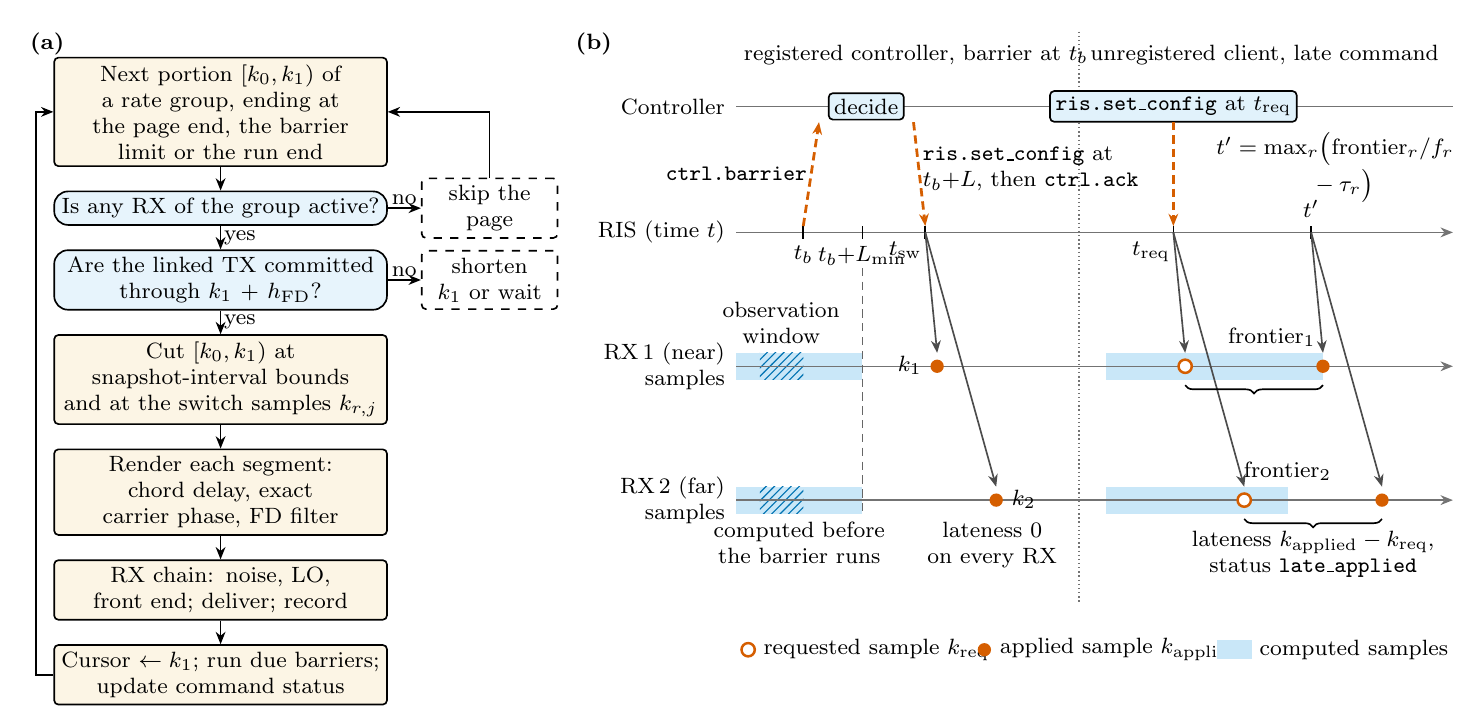
\begin{tikzpicture}[x=1cm, y=1cm, node distance=0.30cm]
  % fixed width: exactly \textwidth of the IEEEtran journal class (43 pc = 516 pt)
  \useasboundingbox (0,0.05) rectangle (516pt,-8.30);

  % ================================================================ (a) pages and segments
  \node[anchor=north west, inner sep=0pt] at (0.02,0) {\figtitle (a)};
  \def\sw{4.05cm}
  \node[step=\sw, anchor=north] (s1) at (2.45,-0.32)
    {Next portion $[k_0,k_1)$ of a rate group, ending at the page end, the barrier limit or
     the run end};
  \node[ask=\sw, below=of s1] (d1) {Is any RX of the group active?};
  \node[ask=\sw, below=of d1] (d2) {Are the linked TX committed through $k_1+h_{\mathrm{FD}}$?};
  \node[step=\sw, below=of d2] (s2)
    {Cut $[k_0,k_1)$ at snapshot-interval bounds and at the switch samples $k_{r,j}$};
  \node[step=\sw, below=of s2] (s3)
    {Render each segment: chord delay, exact carrier phase, FD filter};
  \node[step=\sw, below=of s3] (s4) {RX chain: noise, LO, front end; deliver; record};
  \node[step=\sw, below=of s4] (s5)
    {Cursor $\leftarrow k_1$; run due barriers; update command status};
  \node[side=1.55cm, anchor=west] (n1) at ($(d1.east)+(0.42,0)$) {skip the page};
  \node[side=1.55cm, anchor=west] (n2) at ($(d2.east)+(0.42,0)$) {shorten $k_1$ or wait};
  \draw[flow] (s1) -- (d1);
  \draw[flow] (d1) -- node[right, note, pos=0.5] {yes} (d2);
  \draw[flow] (d2) -- node[right, note, pos=0.5] {yes} (s2);
  \draw[flow] (s2) -- (s3);
  \draw[flow] (s3) -- (s4);
  \draw[flow] (s4) -- (s5);
  \draw[flow] (d1.east) -- node[above, note] {no} (n1.west);
  \draw[flow] (d2.east) -- node[above, note] {no} (n2.west);
  \draw[flow] (n1.north) |- (s1.east);
  \draw[flow] (s5.west) -- ++(-0.22,0) |- (s1.west);

  % ================================================================ (b) command lifecycle
  \node[anchor=north west, inner sep=0pt] at (6.95,0) {\figtitle (b)};
  \def\xl{9.00}  \def\xr{18.10}
  \def\yC{-0.95} \def\yR{-2.55} \def\yA{-4.25} \def\yB{-5.95}
  \node[note, anchor=east, align=right] at (8.90,\yC) {Controller};
  \node[note, anchor=east, align=right] at (8.90,\yR) {RIS (time $t$)};
  \node[note, anchor=east, align=right] at (8.90,\yA) {RX\,1 (near)\\ samples};
  \node[note, anchor=east, align=right] at (8.90,\yB) {RX\,2 (far)\\ samples};

  % samples already computed: before the barrier decides, and before the late command
  \fill[okSky!32] (\xl,\yA-0.17) rectangle (10.60,\yA+0.17);
  \fill[okSky!32] (\xl,\yB-0.17) rectangle (10.60,\yB+0.17);
  \fill[okSky!32] (13.70,\yA-0.17) rectangle (16.45,\yA+0.17);
  \fill[okSky!32] (13.70,\yB-0.17) rectangle (16.00,\yB+0.17);
  % observation window [t_b - W, t_b)
  \fill[pattern=north east lines, pattern color=okBlue] (9.30,\yA-0.17) rectangle (9.85,\yA+0.17);
  \fill[pattern=north east lines, pattern color=okBlue] (9.30,\yB-0.17) rectangle (9.85,\yB+0.17);
  \foreach \y in {\yR,\yA,\yB} { \draw[lane, ->] (\xl,\y) -- (\xr,\y); }
  \draw[lane] (\xl,\yC) -- (\xr,\yC);
  \draw[lane, densely dotted] (13.35,0.0) -- (13.35,-7.25);

  % ---- barrier of a registered controller (lockstep)
  \node[note, anchor=north west] at (9.05,-0.12) {registered controller, barrier at $t_b$};
  \draw (9.85,\yR+0.08) -- (9.85,\yR-0.08) node[below=-1pt] {$t_b$};
  \draw (10.60,\yR+0.08) -- (10.60,\yR-0.08) node[below=-1pt] {$t_b{+}L_{\min}$};
  \draw (11.40,\yR+0.08) -- (11.40,\yR-0.08) node[anchor=north east, inner sep=1pt] {$t_{\mathrm{sw}}$};
  \draw[densely dashed, okBlack!60] (10.60,\yR-0.45) -- (10.60,\yB-0.17);
  \node[note, anchor=south, align=center] at (9.57,\yA+0.24) {observation\\ window};
  \node[note, anchor=north, align=center] at (9.80,\yB-0.24) {computed before\\ the barrier runs};
  \draw[ctrl] (9.85,\yR+0.08) -- node[left, note, pos=0.5] {\texttt{ctrl.barrier}} (10.05,\yC-0.20);
  \node[box, fill=okSky!18, inner sep=2pt] (dec) at (10.65,\yC) {decide};
  \draw[ctrl] (11.25,\yC-0.20) -- node[right, note, pos=0.45, align=left]
    {\texttt{ris.set\_config} at\\ $t_b{+}L$, then \texttt{ctrl.ack}} (11.40,\yR+0.08);
  \draw[okBlack!70, ->] (11.40,\yR) -- (11.55,\yA+0.17);
  \draw[okBlack!70, ->] (11.40,\yR) -- (12.30,\yB+0.17);
  \fill[okVermillion] (11.55,\yA) circle (2.4pt);
  \fill[okVermillion] (12.30,\yB) circle (2.4pt);
  \node[left=2pt] at (11.55,\yA+0.01) {$k_1$};
  \node[right=2pt] at (12.30,\yB+0.01) {$k_2$};
  \node[note, anchor=north, align=center] at (12.25,\yB-0.24) {lateness $0$\\ on every RX};

  % ---- late command of an unregistered source (apply_on_arrival)
  \node[note, anchor=north west] at (13.45,-0.12) {unregistered client, late command};
  \node[box, fill=okSky!18, inner sep=2pt] (cl) at (14.55,\yC) {\texttt{ris.set\_config} at $t_{\mathrm{req}}$};
  \draw[ctrl] (14.55,\yC-0.20) -- (14.55,\yR+0.08);
  \draw (14.55,\yR+0.08) -- (14.55,\yR-0.08) node[anchor=north east, inner sep=1pt] {$t_{\mathrm{req}}$};
  \draw (16.30,\yR+0.08) -- (16.30,\yR-0.08);
  \node[anchor=south] at (16.30,\yR+0.06) {$t'$};
  \node[note, anchor=west, align=left] at (15.05,-1.72)
    {$t'=\max_r\bigl(\mathrm{frontier}_r/f_r$\\ $\qquad\qquad{}-\tau_r\bigr)$};
  \draw[okBlack!70, ->] (14.55,\yR) -- (14.70,\yA+0.17);
  \draw[okBlack!70, ->] (14.55,\yR) -- (15.45,\yB+0.17);
  \draw[okBlack!70, ->] (16.30,\yR) -- (16.45,\yA+0.17);
  \draw[okBlack!70, ->] (16.30,\yR) -- (17.20,\yB+0.17);
  \draw[okVermillion, line width=0.9pt, fill=white] (14.70,\yA) circle (2.4pt);
  \draw[okVermillion, line width=0.9pt, fill=white] (15.45,\yB) circle (2.4pt);
  \fill[okVermillion] (16.45,\yA) circle (2.4pt);
  \fill[okVermillion] (17.20,\yB) circle (2.4pt);
  \node[note, anchor=south east] at (16.40,\yA+0.20) {frontier$_1$};
  \node[note, anchor=south] at (16.00,\yB+0.20) {frontier$_2$};
  \draw[decorate, decoration={brace, amplitude=3pt, mirror}] (14.70,\yA-0.24) -- (16.45,\yA-0.24);
  \draw[decorate, decoration={brace, amplitude=3pt, mirror}] (15.45,\yB-0.24) -- (17.20,\yB-0.24)
    node[midway, below=3pt, note, align=center]
    {lateness $k_{\mathrm{applied}}-k_{\mathrm{req}}$,\\ status \texttt{late\_applied}};

  % ---- legend of panel (b)
  \def\yL{-7.85}
  \draw[okVermillion, line width=0.9pt, fill=white] (9.15,\yL) circle (2.4pt);
  \node[note, anchor=west] at (9.30,\yL) {requested sample $k_{\mathrm{req}}$};
  \fill[okVermillion] (12.15,\yL) circle (2.4pt);
  \node[note, anchor=west] at (12.30,\yL) {applied sample $k_{\mathrm{applied}}$};
  \fill[okSky!32] (15.10,\yL-0.12) rectangle (15.55,\yL+0.12);
  \node[note, anchor=west] at (15.60,\yL) {computed samples};
\end{tikzpicture}
\end{document}
